% 2023.02.14: lecture 01
\documentclass[../main.tex]{subfiles}
\begin{document}

\section{Деревья разбиения}

\subsection{Точки сочленения и блоки в связном графе}

\subsection{Дерево разбиения для набора попарно независимых разделяющих множеств}

\begin{df}[Дерево разбиения] \label{definition:tree_of_partition}
	Пусть $G$ - $k$-связный граф, $\S \subset \R_k(G)$, причем все множества набора $\S$ попарно независимы.

	Тогда \textbf{деревом разбиения} $T(G, \S)$ называется двудольный граф, вершины одной доли $T(G, \S)$ это множества из $\S$, а другой части $\Part(\S)$.

	Вершина $S \in \S$ и $A \in \Part(\S)$ смежны iff $S \subset A$.
\end{df}

\begin{df}
	Пусть $G$ - $k$-связный граф, $\S \subset \R_k(G)$, причем все множества набора $\S$ попарно независимы.

	Тогда граф $G^\S$ это граф $G$ в котором каждое $S \in \S$ дополнили до клики, т.е. провели все пары ребер, которые не присутствовали в $G$.
\end{df}

\begin{lm}[Лемма 1.1] \label{lemma:1_1}
	Выполняется: $\S \subset \R_k(G^\S)$.

	Более того, $\Part(G; \S) = \Part(G^\S, \S)$.
\end{lm}

\begin{proof}
	Понятно, что если две вершины разделены в $G^\S$, то они разделены и в $G$.

	В обратную сторону, если вышло так что вершины $a, b$ отделены каким то множеством $S \in \S$ в  $G$, а в  $G^\S$ все равно существует путь после удаления $S$, то тогда можно сказать что этот путь проходит в какой то момент по ребру  $(c,d) \in E(G^\S) \setminus E(G)$ и при этом не существует пути $cd$ по ребрам $E(G)$(ведь тогда это ребро на пути можно заменить целиком путем из $E(G)$).
	А значит получили что вершины $c, d$ отделены множеством $S$, противоречие с попарной независимостью элементов  $\S$.
\end{proof}

\begin{lm}[Лемма 1.2] \label{lemma:1_2}
	Пусть $G$ - $k$-связный граф, $\S \subset \R_k(G)$ и все множества $\S$ попарно независимы.

	Тогда для произвольного $\T \subset \S, B \in \Part(G; \T)$ и $R \in \R(G^\S(B))$ такого что, $R$ не содержит рёбра, соединяющие пары вершин, входящих в какое-либо множество набора $\S$.
	
	Тогда $R \in \R(G)$.

	В частности, граф  $G^\S(B)$ является $k$-связным.
\end{lm}

\begin{proof}

	Предположим, что $R \not \in \R(G)$.

	Пусть $x, y \in B$ и множество  $R$ отделяет $x$ и $y$ в $G^\S(B)$, но не отделяет в $G$.
	Тогда по лемме \ref{lemma:1_1} $R$ не отделяет $x$ и $y$ и в $G^\S$.

	Тогда рассмотрим кратчайший путь  $xy$ в $G^\S - R$, назовем этот путь $P$.

	Предположим что путь $P$ содержит $z \not \in B$, но тогда существует $T \in \T$, которое отделяет $z$ от $B$.
	Тогда двигаясь по пути $P$ мы как минимум дважды войдем в $T$, обозначим эти вершины $a, b$.

	По условию $ab \not \in R$, а следовательно в $G^\S$ есть ребро $(a,b)$.
	Значит можно выкинуть кусок пути и укоротить путь.
	Рисунок \ref{fig:lemma_1_2}.

\begin{figure}[ht]
    \centering
	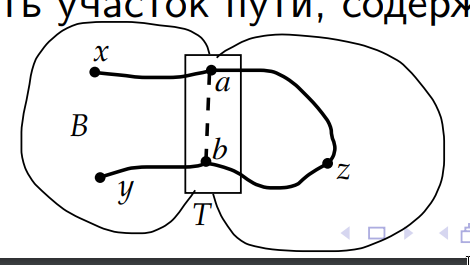
\includegraphics[width=0.3\columnwidth]{figures/lemma_1_2.png}
    \caption{Рисунок к лемме \ref{lemma:1_2}}
    \label{fig:lemma_1_2}
\end{figure}

	Отсюда следует что $P \subset B$, значит $P$ путь в  $G^\S(B) - R$, но такого пути нет ведь $R$ разделяет $x$ и $y$.
	Следовательно, $R \in \R(G)$.

	В завершении добавим, что $\R_{k-1}(G) = \varnothing$, а значит и  $\R_{k - 1}(G^\S(B)) = \varnothing$, следовательно $G^\S(B)$ - $k$-связный.
	
\end{proof}

\begin{thm}[Теорема 1.1] \label{theorem:1_1}
	Пусть $G$ -  $k$-связный граф, $\S \subset \R_k(G)$ - набор попарно независимых множеств.
	Тогда выполняются следующие утверждения:

	 \begin{enumerate}
		 \item $\wT(G, \S)$ - это дерево \label{stmt:theorem_1_1_1}
		 \item Для каждого множества $S \in \S$ выполняется  $d_{\wT(G, \S)}(S) = |\Part(S)|$.
			 Более того, для каждой части  $A \in \Part(S)$ существует единственная часть  $B \in \Part(\S) \colon B \subset A$ и  $B$ смежна с  $S$ в  $\wT(G, \S)$ \label{stmt:theorem_1_1_2}
		 \item Все висячие вершины дерева  $\wT(G, \S)$ соответствуют частям  $\Part(\S)$ \label{stmt:theorem_1_1_3}
		 \item Множество  $S$ разделяет части  $B, B' \in \Part(\S)$ в графе  $G \iff$ когда  $S$ разделяет  $B, B'$ в  $T(G, \S)$ \label{stmt:theorem_1_1_4}
	\end{enumerate}
	
\end{thm}

\begin{proof}
	Заметим, что Утверждение \eqref{stmt:theorem_1_1_3} следует из Утверждения \eqref{stmt:theorem_1_1_2}.

	Рассмотрим  $G^* = G^\S$.
	По Лемме \ref{lemma:1_1} следует, что разбиения графов  $G$ и  $G^*$ набором  $\S$ совпадают. Обозначим это разбиение за  $\Part(\S)$.

	Тогда  $T(G, \S) = T(G^*, \S)$, поэтому докажем утверждения теоремы для графа  $G^*$.

	Пусть $S \in \S, \Part(S) = \{A_1, \ldots, A_n\}, G_i = G^*(A_i)$.
	По Лемме \ref{lemma:1_2} все графы $G_1, \ldots, G_n$ являются  $k$-связными.

	Пусть набор  $\S_i$ состоит из всех множеств набора  $\S$, лежащих в  $A_i$ и отличных от  $S$.

	Тогда каждое множество из  $\S \setminus \{S\}$ лежит ровно в одном из наборов $\S_1, \ldots, \S_n$.

	Для каждого $i$ пусть $U_i \in \Part(G_i;\S_i)$ - часть, содержащая  $S$.
	По Лемме \ref{lemma:1_2}, для любой части $U \in \Part(G_i;\S_i)$ граф $G^*(U)$ является  $k$-связным, а значит, его не разделяет ни одно из множеств набора  $\S$, не лежащих в  $U$. 

	Множество $S$ лежит в части  $U_i$, но также не разделяет ее, т.к. $U_i \subset A_i \in \Part(G;S)$.
	Это означает, что  $\Part(G_i;\S_i) \subset \Part(G^*; \S)$, причем именно  $U_i$ содержит  $S$.

	Следовательно, $\Part(G^*; \S) = \bigcup\limits_{i=1}^n \Part(G_i;\S_i)$, причем объединение дизъюнктное, а части  $\Part(\S)$, содержащие множество  $S$ - это  $U_1, \ldots, U_n$.
	Таким образом Утверждения \eqref{stmt:theorem_1_1_2} и \eqref{stmt:theorem_1_1_4} доказаны для множества  $S$, для остальных множеств из  $\S$ доказательство аналогично.

\begin{figure}[ht]
    \centering
	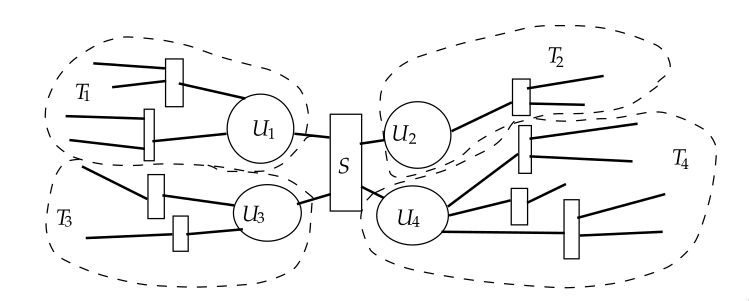
\includegraphics[width=0.5\columnwidth]{figures/theorem_1_1.png}
    \caption{Рисунок к Теореме \ref{theorem:1_1}}
    \label{fig:theorem_1_1}
\end{figure}

	Чтобы показать Утверждение \eqref{stmt:theorem_1_1_1}, воспользуемся индукцией по количеству элементов в наборе $\S$ и при это не фиксируем  $k, G$.
	Теперь скажем что каждая часть $\Part(G_i; \S_i)$, кроме  $U_i$ смежна в  $T_i = T(G_i, \S_i)$ с теми же вершинами, что в  $T(G, \S)$.
	Для части  $U_i$ в  $T(G, \S)$ добавляется ребро к множеству  $S$.

	Поэтому  $T(G, \S) - S$ распадается ровно на  $n$ связных подграфов: это графы  $T_i$, где  $i \in [n]$.
	По индукционному предположению, все эти графы - деревья.

\end{proof}

\subsection{Дерево разрезов}

\subsection{Гипердерево}

\subsection{Гипердерево разбиения $\Struct(V)$}

\todo[inline]{Дописать лекцию 1}

\end{document}
